\chapter{Design}

\section{Application Architecture}
The application has inside both client and server components bacause, being this a end-to-end encrypted command system it's mandatory to avoid to rely on an external server which would have required the usage of ssl which we planned to avoid prom the beginning (we absolutely didn't want to introduce (un)trusted elements). The client part allows the user to actively use alla the functionalities, while the server one silently receives the messages from other telephones, parses them and reacts to them in the proper way.

\section{Design Patterns}
In order to ensure scalability and order in the SMP and command architectures a visitor pattern has been employed: the system "visits" the received message in a different method of a different class depending on his header (See the class diagrams below for a visual explaination). We also decided to catch the exceptions at the highest level possible, because this way it was easier to implement better errors reaction policies which informs the user of the internal error(s).
\newpage
\section{Class diagrams}

\begin{center}
\textbf{SMP diagram}\\
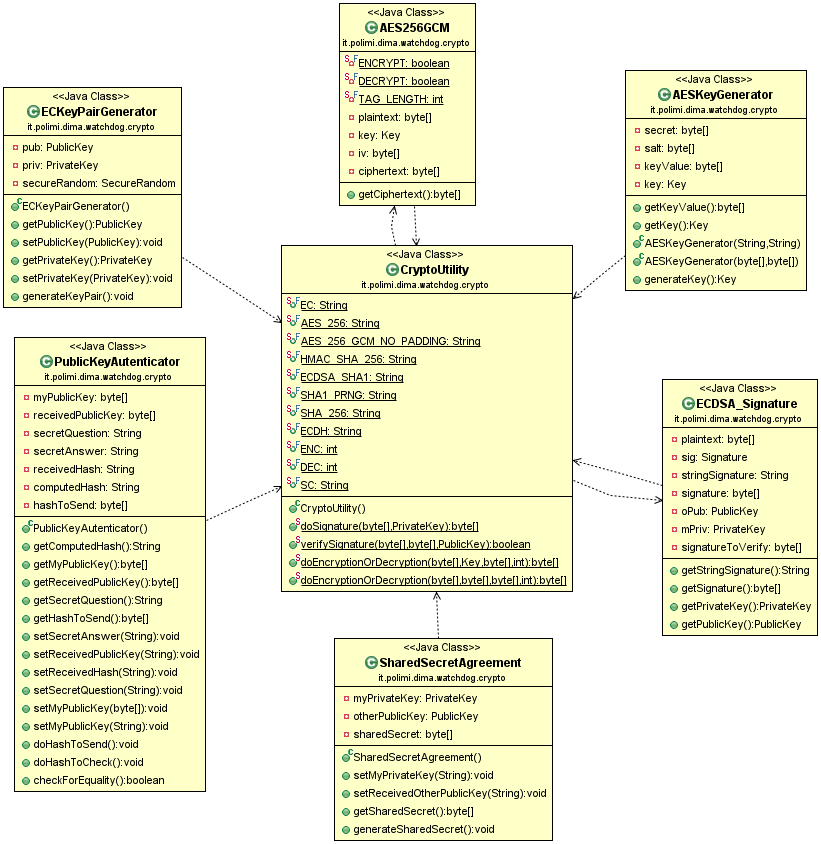
\includegraphics[scale=0.5]{images/smp}
\end{center}
\newpage
\begin{center}
\textbf{Commands diagram}\\
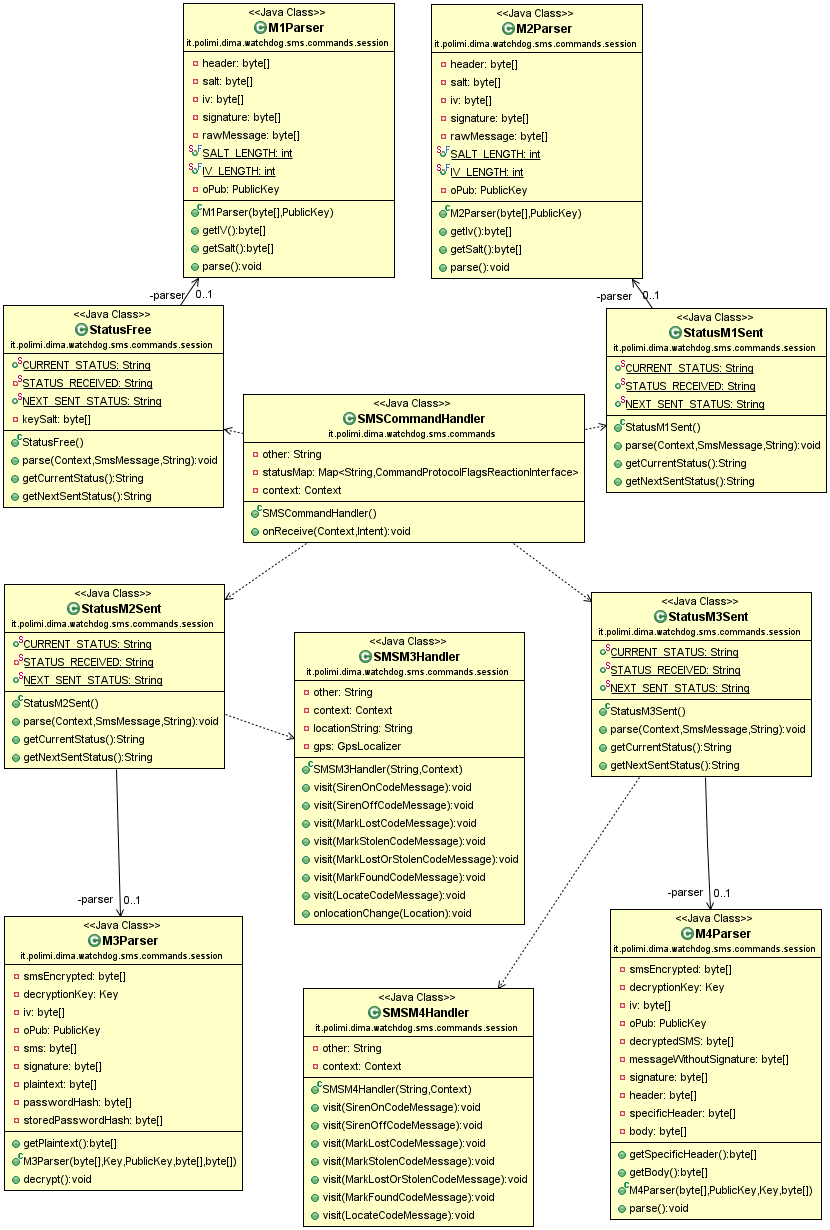
\includegraphics[scale=0.45]{images/commands}
\end{center}
\newpage
\begin{center}
\textbf{Cryptography diagram}\\
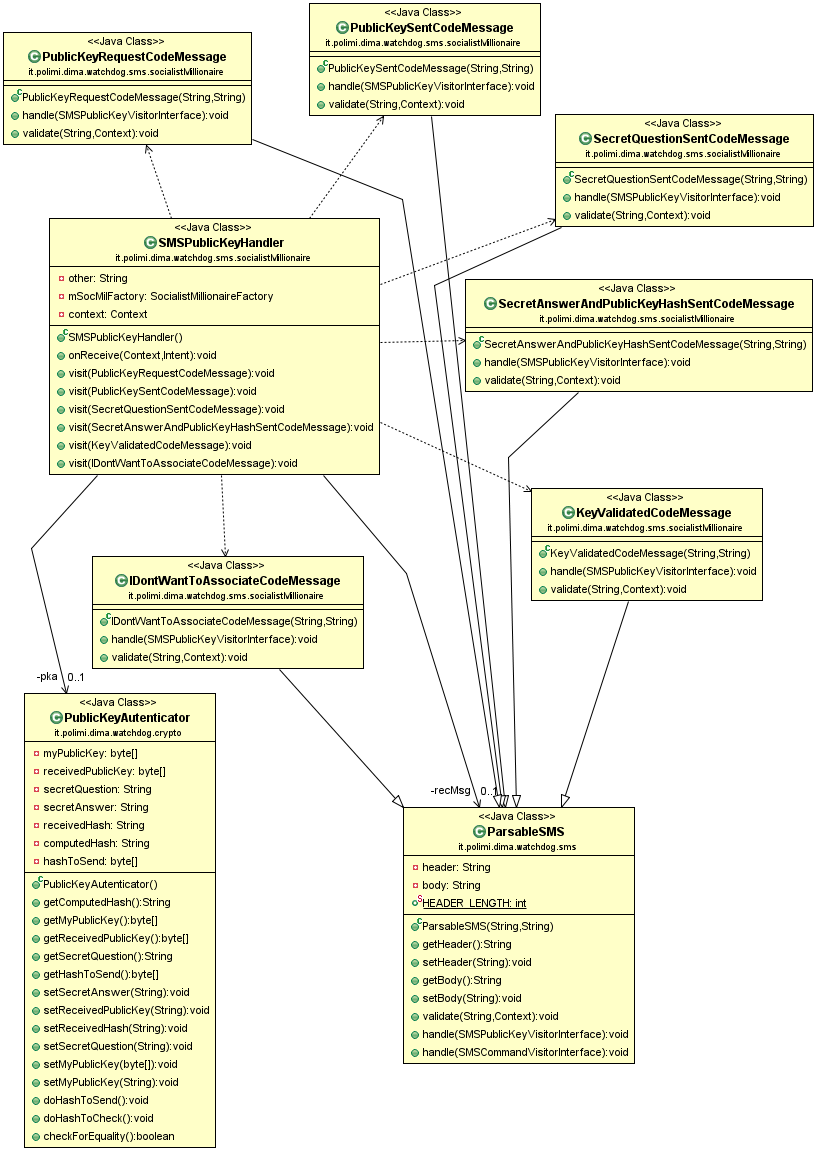
\includegraphics[scale=0.5]{images/crypto}
\end{center}
\newpage